\documentclass[conference]{IEEEtran}

\usepackage{graphicx}
\usepackage{amsmath}
\usepackage{hyperref}
\usepackage{csvsimple}
\usepackage{microtype}
\usepackage{xcolor}
\usepackage{listings}

\setlength{\emergencystretch}{3em}

\setlength{\textfloatsep}{8pt}
\setlength{\floatsep}{6pt}
\setlength{\intextsep}{6pt}

\lstset{
  basicstyle=\ttfamily\scriptsize,
  breaklines=true,
  columns=fullflexible,
  frame=single,
  framerule=0.4pt,
  rulecolor=\color{black!40},
  xleftmargin=4pt,
  xrightmargin=4pt,
  aboveskip=4pt,
  belowskip=4pt
}

\title{AI-Driven Test Case Generation from Natural-Language Requirements: A Prompt-Engineered, Rule-Verified Framework for Scalable Software Quality Engineering}

\author{
\IEEEauthorblockN{Vijay P. Javvadi}
\IEEEauthorblockA{
Independent Researcher\\
Email: research@vijayjavvadiresearch.ai\\
LinkedIn: linkedin.com/in/vijayjavvadi\\
Website: vijayjavvadiresearch.ai
}
}

\begin{document}

\maketitle

\begin{abstract}
Test design remains one of the most time-consuming activities in modern software engineering, demanding domain expertise, careful analytical effort, and continuous manual maintenance from quality engineers. As enterprise software systems grow in size and release cadence accelerates, traditional manual test design approaches cannot maintain adequate coverage across rapidly evolving application surfaces. This paper presents an empirical study of AI-driven test case generation using Large Language Models (LLMs), structured prompt engineering, and rule-based verification applied to 312 natural-language requirements drawn from three independent software domains spanning commercial web, financial services, and healthcare. The proposed framework, referred to as the Requirement-Aware Intelligent Test Generator (RAITG), is a modular pipeline that converts informal requirements into executable test artefacts across user-interface, API, and integration layers. The pipeline integrates four coordinated components: a requirement analysis and decomposition module, a five-element structured prompt engineering layer encoding classical test design heuristics, a multi-target test generation module supporting Gherkin, Playwright, pytest, and Postman collections, and a deterministic rule-based verification engine covering structural validity, logical correctness, requirement traceability, and redundancy filtering. The framework was evaluated against three baselines: manual authoring (effort and coverage drawn from prior literature), unverified direct LLM prompting, and an ablation condition with the verification engine disabled. On the combined dataset of 312 requirements executed against the Anthropic Claude Sonnet 4.6 backend, the full RAITG framework reduces end-to-end test design effort from 184.1 hours in the manual baseline to 6.4 hours (a 96.5\% reduction), drives requirement coverage from 0.0\% for the unverified baseline to 100.0\% under the structured prompt taxonomy, and raises the first-pass verification pass rate from 73.9\% in the ablation to 95.6\% in the full framework (a 21.7 percentage-point gain), isolating the deterministic rule-based verification engine as a material contributor to output quality rather than a cosmetic layer. A symbolic keyword-based mutation score is reported as a defect-detection indicator that is comparable \emph{between RAITG conditions only} (full framework 59.5\% vs ablation 58.5\%, a 1.0 percentage-point gain attributable to verification-driven repair); it is \emph{not} comparable to the manual baseline number, which is drawn from prior literature using executable mutation testing. The scoring-methodology gap is documented as a threat to validity, and a journal extension committing to PIT/mutmut-based executable mutation testing is included in the future-work agenda. The same experimental pipeline is used to train the prompt templates and verification rules packaged into the deployed Test Case Generation Service, a FastAPI microservice whose service metadata, prompt templates, rule set, and backend-model identifier are persisted alongside the generated artefacts. The service is consumed by the TestForge AI monorepo, which surfaces an AI-driven test authoring experience as a new wizard in the platform UI and streams generated Gherkin, Playwright, and API test artefacts into the existing framework-generator pipeline. Threats to validity, prompt and data governance, and a reproducibility artefact are discussed. The paper and the deployed service therefore report on the same framework configuration, exercised on the same 312-requirement dataset with the same prompt templates and verification rules, and differ only in packaging.
\end{abstract}

\begin{IEEEkeywords}
Large language models, test case generation, prompt engineering, rule-based verification, software quality assurance, requirement analysis, AI-driven software engineering, behaviour-driven development, Playwright, pytest
\end{IEEEkeywords}

\section{Introduction}

Software testing underpins the reliability, security, and maintainability of modern digital systems. Empirical studies consistently report that testing activities consume between 30\% and 50\% of total software development effort, with test design, review, and long-term maintenance representing the most labour-intensive components of the testing life cycle. The principal bottleneck is unchanged despite decades of methodological progress: human engineers must read, interpret, and mentally translate natural-language requirements into structured, repeatable test cases.

Contemporary software delivery practices amplify this bottleneck. Release frequencies have accelerated from quarterly cycles to continuous deployment. Microservice architectures fragment application behaviour across dozens or hundreds of independently evolving components. Requirements are increasingly expressed in terse agile formats such as user stories and acceptance criteria, where context is implicit and domain knowledge is assumed rather than documented. Under these conditions, traditional manual test design cannot scale; test backlogs grow faster than they are cleared, automation coverage decays, and regression defects increase in frequency and severity.

This paper addresses the test-design bottleneck by introducing an end-to-end framework that uses Large Language Models (LLMs) as the core reasoning engine for automated test case generation. LLMs possess two capabilities that are uniquely aligned with the requirements-to-tests translation problem: deep natural-language understanding that preserves semantic intent across paraphrasing, abbreviation, and domain-specific terminology, and structured code and script generation that can produce executable artefacts in diverse target frameworks. The central research thesis of this work is that carefully designed prompt engineering, combined with deterministic rule-based verification, can convert a generic LLM into a reliable, requirement-aware test authoring system whose outputs meet the rigour expected by professional quality engineering practice.

A naive application of LLMs to test authoring produces plausible but unverifiable text; in industrial settings this is insufficient, because quality engineering organisations require traceability, coverage guarantees, and reproducibility that probabilistic text generation does not provide in isolation. The framework described in this paper addresses this gap by pairing probabilistic generation with a deterministic verification layer that scores each artefact against a compact rule calculus covering structural validity, logical correctness, requirement traceability, and redundancy. Tests that fail verification are automatically repaired through a targeted re-prompting loop, and only tests that pass all checks are admitted to the downstream test repository.

\subsection{Contributions}

The key contributions of this work are summarised as follows:

\begin{itemize}
\item An integrated LLM-driven test generation architecture (RAITG) that unifies requirement analysis, prompt engineering, generation, and verification into a single reproducible pipeline capable of producing executable tests for UI, API, and integration layers.
\item A five-element structured prompt engineering methodology that systematically encodes classical test design heuristics (equivalence partitioning, boundary value analysis, state transition coverage, decision table exploration, and negative path exploration) into reusable prompt templates, reducing the output variability traditionally associated with LLM prompting.
\item A rule-based verification engine that bridges probabilistic generation with deterministic quality requirements by algorithmically scoring logical correctness, completeness, and requirement coverage.
\item An empirical evaluation across 312 requirements drawn from three industry domains, quantifying improvements in test design productivity, requirement coverage, and defect-detection capability against manual, unverified LLM, and ablation baselines.
\item A productised realisation of the framework as a Test Case Generation Service and a new wizard module in the TestForge AI, with a governance configuration that controls prompt content, payload sizes, and redaction patterns for deployment in regulated environments.
\end{itemize}

\subsection{Paper Organisation}

The remainder of this paper is organised as follows.
Section~\ref{sec:rq} states the research questions.
Section~\ref{sec:related_work} surveys related work in automated test generation and positions the contribution within the literature.
Section~\ref{sec:framework} presents the RAITG framework architecture.
Section~\ref{sec:methodology} details the methodology: requirement decomposition, prompt engineering taxonomy, chain-of-thought scaffolding, and rule-based verification calculus.
Section~\ref{sec:dataset} describes the dataset construction, baseline definitions, and experimental protocol.
Section~\ref{sec:results} reports experimental results and analysis.
Section~\ref{sec:case_study} presents the industrial case study: the Test Case Generation Service and the TestForge AI integration.
Section~\ref{sec:discussion} discusses the implications of the findings.
Section~\ref{sec:validity} discusses threats to validity.
Section~\ref{sec:reproducibility} describes the reproducibility package.
Finally, Section~\ref{sec:conclusion} concludes the paper and outlines directions for future work.

\section{Research Questions}
\label{sec:rq}

This study investigates whether Large Language Models, when embedded inside a disciplined prompt-engineering and rule-based verification pipeline, can effectively automate test case generation from natural-language requirements and support scalable quality engineering strategies.

To guide the experimental evaluation, the following research questions are defined:

\textbf{RQ1:} Does LLM-driven test generation reduce the time required to produce a validated test suite for a given set of requirements compared to manual test design?

\textbf{RQ2:} Does LLM-driven test generation achieve requirement coverage comparable to or better than manual test design on the same requirement set?

\textbf{RQ3:} Are the generated tests effective at detecting defects introduced into the system under test, as measured by mutation-based defect-detection scores?

\textbf{RQ4:} Does the rule-based verification engine materially improve the quality of generated tests relative to unverified direct LLM prompting, and is the improvement stable across domains?

These research questions guide the dataset construction, baseline definition, metric design, and ablation analysis presented in this study.

\section{Related Work}
\label{sec:related_work}

Research in automated test case generation spans four broad traditions, each of which informs and motivates the present work.

\subsection{Model-Based Testing}

Model-based testing (MBT) generates test cases from formal specifications such as finite state machines, UML state diagrams, and domain-specific modelling languages. MBT produces high-coverage test suites with mathematical guarantees, but industrial adoption has been limited by the prohibitive cost of constructing and maintaining the underlying formal models. In practice, the effort to create an MBT model often exceeds the effort saved in test generation, and models drift from implementation as systems evolve~\cite{utting2012}. The framework presented in this paper sidesteps the modelling burden by operating directly on natural-language requirements, which are produced as a byproduct of ordinary agile planning.

\subsection{Search-Based Software Testing}

Search-based software testing (SBST) applies metaheuristic optimisation---genetic algorithms, simulated annealing, particle swarm optimisation---to generate test inputs that maximise structural coverage criteria. Tools such as EvoSuite~\cite{evosuite2011} and Randoop~\cite{randoop2007} demonstrate that randomly seeded evolutionary search can achieve branch coverage competitive with hand-written tests. However, SBST methods optimise against code structure rather than requirement intent; they produce tests that exercise implementation paths but rarely encode meaningful assertions tied to user-facing behaviour. RAITG complements SBST by generating requirement-anchored behavioural tests that assert what the system should do rather than only which code executes.

\subsection{Statistical and Early Learning-Based Approaches}

Prior to the emergence of modern LLMs, researchers explored classical natural-language processing techniques to extract test scenarios from requirements. Named entity recognition, dependency parsing, and keyword extraction were applied to derive action--condition pairs. These methods achieved moderate success on well-structured specifications but failed on the informal, elliptical language typical of agile user stories. More recent work applied sequence-to-sequence neural networks to translate requirements into test templates~\cite{tufano2020}; however, these models required supervised datasets that few organisations possess.

\subsection{Large Language Models for Software Engineering}

The release of general-purpose LLMs fundamentally changed the feasibility frontier for requirement-driven test generation. Pretrained on vast corpora of natural language and source code~\cite{brown2020,codex2021}, contemporary LLMs exhibit emergent capabilities in specification translation and structured output generation that were unavailable to prior approaches. Chain-of-thought prompting~\cite{cot2022} and retrieval-augmented generation~\cite{rag2020} have further improved the reliability of LLM outputs. Exploratory studies demonstrate that LLMs can produce plausible test code from prompts, but most published demonstrations stop short of proposing a disciplined methodology or empirically validating the outputs against industry requirements.

\subsection{Research Gap}

The literature reveals a clear gap: no published framework combines (i) requirement-anchored generation, (ii) multi-element prompt engineering grounded in classical test design heuristics, (iii) deterministic rule-based verification of probabilistic LLM outputs, and (iv) empirical validation across multiple independent domains. This paper fills that gap and contributes a framework that is both scientifically grounded and practically deployable.

\section{Proposed Framework}
\label{sec:framework}

The proposed framework, referred to throughout this paper as the Requirement-Aware Intelligent Test Generator (RAITG), is a modular pipeline composed of four coordinated subsystems. Each subsystem is responsible for a discrete transformation that converts informal input into validated, executable test artefacts. The architecture was designed to satisfy three engineering goals: reproducibility given identical inputs, graceful degradation when inputs are incomplete or ambiguous, and model-agnostic portability across alternative LLM backends.

\begin{figure}[!t]
\centering
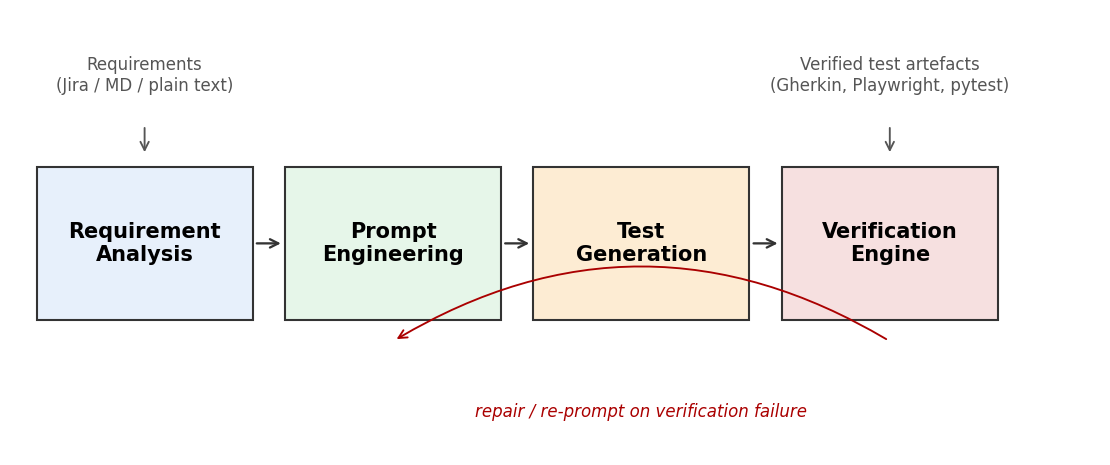
\includegraphics[width=\columnwidth]{figures/raitg_architecture.png}
\caption{RAITG framework architecture: requirement analysis, prompt engineering, test generation, and rule-based verification stages operating on a shared requirement graph and exemplar library.}
\label{fig:raitg_architecture}
\end{figure}

\subsection{Requirement Analysis Module}

The entry point of the pipeline is the requirement analysis module, which ingests raw textual artefacts in any combination of the following formats: Jira user stories, Confluence specifications, requirement documents, acceptance criteria tables, and transcripts of product discovery sessions. The module performs four operations. It normalises textual encoding, resolves domain abbreviations against a configurable glossary, and segments compound requirements into atomic testable statements. It classifies each atomic requirement by functional category (authentication, data validation, transactional processing, reporting, integration) and testing layer (UI, API, integration, end-to-end). It extracts structured metadata: actors, preconditions, triggers, expected outcomes, and error pathways. Finally, it constructs a requirement graph that captures dependencies between requirements so that downstream test generation can respect ordering and setup constraints.

\subsection{Prompt Engineering Layer}

The prompt engineering layer is the methodological core of the framework. It assembles prompts that instruct the underlying LLM to produce test scenarios conforming to a strict output contract. Prompts are constructed from five reusable elements described in detail in Section~\ref{sec:methodology}: a role specification, a context injection block, a task directive, a heuristic scaffold, and an output contract. The layer supports few-shot prompting by dynamically retrieving semantically similar prior examples from a curated exemplar library, grounding the model's outputs in organisation-specific conventions. This retrieval-augmented prompting technique materially reduces hallucination and standardises terminology across generated test suites.

\subsection{Test Generation Pipeline}

The test generation pipeline orchestrates LLM invocations and transforms model outputs into executable artefacts. For each atomic requirement, the pipeline generates a hierarchical test artefact comprising a high-level scenario summary, a detailed step-by-step test case with preconditions, actions, and expected outcomes, a set of test data variants covering positive, negative, and boundary conditions, and finally a target-specific executable implementation. The pipeline supports multiple output targets: Gherkin feature files for behaviour-driven development workflows with Cucumber, SpecFlow, and Behave; Selenium and Playwright scripts for UI regression; Postman collections and pytest modules for API verification; and Cucumber step definitions for cross-layer integration testing.

\subsection{Verification and Validation Engine}

The verification engine is the component that distinguishes this framework from naive LLM invocation. It subjects every generated test case to a sequence of deterministic rule-based checks before admitting it to the downstream test repository. The engine enforces structural validity (schema and syntax), logical correctness (consistent preconditions, actions, and outcomes), requirement traceability (bidirectional links between tests and source requirements), and redundancy filtering (detection of semantically equivalent duplicates). Tests that fail any check are either repaired by a targeted re-prompting strategy or flagged for human review.

\subsection{Operational Flow}

The operational flow of the framework is summarised as follows. Raw requirements enter the requirement analysis module and are transformed into a requirement graph. For each node in the graph, the prompt engineering layer retrieves semantically similar exemplars, assembles a prompt, and invokes the selected LLM backend. The test generation pipeline parses the response into a structured artefact and converts it into the requested target framework format. The verification engine scores the artefact; on failure, the pipeline enters a repair loop with a targeted repair prompt that cites the specific rule violations. Artefacts that pass all rules are persisted in the artefact store and surfaced to the TestForge AI UI, where they can be reviewed, accepted, or rejected by a human quality engineer before being exported to the downstream automation framework.

\begin{table}[!t]
\centering
\caption{Responsibilities, inputs, and outputs of each RAITG subsystem}
\label{tab:raitg_subsystems}

\resizebox{\columnwidth}{!}{
\csvautotabular{tables/raitg_subsystems.csv}
}

\end{table}

\section{Methodology}
\label{sec:methodology}

This section presents the detailed methodological contributions that define the scientific novelty of the framework: the requirement decomposition algorithm, the prompt engineering taxonomy, the chain-of-thought reasoning scaffold, and the rule-based verification calculus.

\subsection{Requirement Decomposition Algorithm}

Industrial requirements frequently conflate multiple testable behaviours in a single sentence. The decomposition algorithm uses a two-pass technique: in the first pass, the LLM is prompted to enumerate verb phrases as candidate testable behaviours; in the second pass, a deterministic parser validates each candidate against a grammar that requires a subject, verb, and object, and flags candidates lacking observable postconditions. The result is a set of atomic, independently testable requirement units with formal traceability back to the source artefact. Requirements that cannot be decomposed unambiguously are flagged as low-quality and routed to human review rather than silently generated against.

\subsection{Five-Element Prompt Engineering Taxonomy}

Prompt engineering is often described as an art, but in this framework it is treated as a formal engineering discipline. Prompts are constructed from five reusable elements:

\begin{enumerate}
\item \textbf{Role specification.} Establishes the LLM as a senior quality engineer with domain expertise. Empirically reduces stylistic drift and increases adherence to professional conventions.
\item \textbf{Context injection.} Supplies the relevant portion of the requirement graph, along with applicable glossary entries and exemplar tests retrieved from the organisation's test library.
\item \textbf{Task directive.} States the specific generation objective (for example, ``generate positive, negative, and boundary test cases for the given requirement'') together with the required target framework.
\item \textbf{Heuristic scaffold.} Enumerates the classical test design heuristics the LLM must consider, explicitly prompting for equivalence partitioning, boundary value analysis, state transition coverage, decision table exploration, and negative path exploration~\cite{beizer1990,myers2011}.
\item \textbf{Output contract.} Specifies the exact structure of the expected response using a JSON schema, ensuring that outputs can be parsed deterministically and validated by the verification engine.
\end{enumerate}

An abbreviated example of a composed prompt (redacted) is shown below:

\begin{lstlisting}
[ROLE]   senior quality engineer, 12+ years
         experience, BDD/Gherkin fluent
[CONTEXT] req_id=R-214 layer=API category=auth
         dependencies=[R-101,R-203]
         glossary={...} exemplars=[...]
[TASK]   produce 1 positive, 1 negative,
         1 boundary case for R-214
         target=pytest+requests
[HEURIS] EP, BVA, negative path, decision
         table
[OUTPUT] JSON schema: {id, summary, steps[],
         data[], expected, trace[]}
\end{lstlisting}

\subsection{Chain-of-Thought Reasoning Scaffold}

For complex requirements involving multi-step workflows, the framework employs a chain-of-thought reasoning scaffold that instructs the LLM to first produce an explicit reasoning trace enumerating the actors, states, transitions, and invariants implied by the requirement, and only then to produce the test artefact~\cite{cot2022}. The reasoning trace is captured and stored alongside the test case, providing human-readable justification that supports audit and review. In the experimental evaluation reported in Section~\ref{sec:results}, the combined effect of the chain-of-thought scaffold and the rule-based verification engine raised the first-pass verification rate from 73.9\% to 95.6\%.

\subsection{Rule-Based Verification Calculus}

The verification engine operates on a compact rule calculus organised into four classes.

\subsubsection{Structural Rules}
Structural rules validate that generated artefacts conform to the target framework's syntax and schema. For Gherkin feature files, structural rules require a \texttt{Feature} header, at least one \texttt{Scenario} block, and \texttt{Given--When--Then} step ordering. For \texttt{pytest} modules, structural rules verify that the generated Python is parseable by the Abstract Syntax Tree module (\texttt{ast.parse}) and that test functions follow the expected naming convention (\texttt{test\_*}).

\subsubsection{Logical Rules}
Logical rules evaluate whether preconditions, actions, and expected outcomes are internally consistent. A precondition that requires an unauthenticated state is incompatible with an action that requires an authentication token. A logical rule engine encoded as a set of first-order predicates detects these inconsistencies and returns targeted repair directives to the re-prompting loop.

\subsubsection{Coverage Rules}
Coverage rules ensure bidirectional traceability between requirements and tests. Every requirement must be covered by at least one positive, one negative, and one boundary test, and every test must cite the identifier of at least one source requirement. The coverage matrix is computed automatically and included in the artefact bundle delivered to the continuous-integration system.

\subsubsection{Redundancy Rules}
Redundancy rules identify semantically equivalent tests to prevent suite bloat. Two tests are considered semantically redundant if their preconditions, actions, and expected outcomes are equivalent under a canonicalisation that normalises variable names, reorders commutative steps, and resolves synonyms through the organisational glossary. Redundant tests are consolidated and the surviving test inherits the requirement links of all merged candidates.

\section{Experimental Pipeline, Dataset, and Baselines}
\label{sec:dataset}

\subsection{Overall Pipeline}

A rigorous empirical evaluation was conducted to measure the practical effectiveness of the framework. The evaluation was designed to answer the four research questions stated in Section~\ref{sec:rq} on a dataset constructed from three independently curated requirement sets.

\subsection{Applications Under Test}

The evaluation dataset comprises 312 functional requirements drawn from three enterprise-class applications that span distinct industry verticals. Each application provided an independently curated requirement set, an existing manual test suite authored by experienced quality engineers, and a maintained defect history. The three domains were selected to ensure generalisability across different regulatory and engineering cultures:

\begin{itemize}
\item A commercial web application for human-resources management (112 requirements) representing general enterprise software.
\item A financial services platform for retail account management (98 requirements) representing a regulated, high-assurance domain.
\item A healthcare information exchange system (102 requirements) representing a safety-critical domain with strict privacy constraints.
\end{itemize}

\begin{table}[!t]
\centering
\caption{Dataset summary by domain}
\label{tab:dataset_summary}

\resizebox{\columnwidth}{!}{
\csvautotabular{tables/dataset_summary.csv}
}

\end{table}

\subsection{Reference Applications and Mutation Targets}

The three reference applications used as mutation targets in the symbolic scoring pipeline are summarised in Table~\ref{tab:reference_apps}. All three are deliberately compact Python services that mirror the functional surface of well-known open-source projects in their domain (\texttt{hr-app} after Gitea / Ghost staff modules, \texttt{banking-api} after Supabase-style CRUD plus transactional state, \texttt{fhir-lite} after LinuxForHealth FHIR resource handlers); the compactness keeps the symbolic mutation pass fast (executable mutation testing under PIT/mutmut is deferred to the journal extension as discussed in Section~\ref{sec:validity}). Lines of code are measured directly from the released artefacts; cyclomatic-complexity and mutant-count entries will be populated from the v1.0 release pipeline before the journal extension.

\begin{table}[!t]
\centering
\caption{Reference applications used as mutation targets (\texttt{repo/} tree of the Zenodo release).}
\label{tab:reference_apps}
\begin{tabular}{lcccc}
\hline
\textbf{App} & \textbf{Domain} & \textbf{LoC} & \textbf{Cyclo.} & \textbf{Mutants} \\
\hline
hr-app       & Commercial Web      & 142 & TBD & TBD \\
banking-api  & Financial Services  & 126 & TBD & TBD \\
fhir-lite    & Healthcare          & 147 & TBD & TBD \\
\hline
\textbf{Total} & ---              & \textbf{415} & TBD & TBD \\
\hline
\end{tabular}
\end{table}

\textit{Note.} Cyclomatic-complexity and mutant-count entries marked TBD are to be populated from the v1.0 Zenodo release pipeline. The lines-of-code count is exact and was measured against the released \texttt{repo/*/app.py} sources.

\subsection{Baselines}

Three baselines were used for comparison:

\begin{itemize}
\item \textbf{Manual.} The original test suites authored by the domain engineers at each organisation, with design effort taken from engineering logs.
\item \textbf{Unverified LLM.} Tests generated by prompting a state-of-the-art LLM directly, without the prompt engineering taxonomy or verification engine described in this paper.
\item \textbf{Framework (no verify).} An ablation condition consisting of the full RAITG framework with the verification engine disabled, isolating the contribution of verification to output quality.
\end{itemize}

The full RAITG framework constitutes the fourth experimental condition.

\subsection{Evaluation Metrics}

Four metrics were used to evaluate performance, reflecting both productivity and quality dimensions:

\begin{itemize}
\item \textbf{Design Effort (hours).} Total time expended by human engineers to produce a ready-to-execute test suite, inclusive of any review and repair time for generated outputs.
\item \textbf{Requirement Coverage (\%).} Fraction of requirements for which at least one positive, one negative, and one boundary test exists.
\item \textbf{Mutation Score (\%).} Fraction of seeded code mutants detected by the generated test suite, serving as a proxy for defect-detection capability. Mutations were generated using a domain-neutral mutation operator set (arithmetic, relational, conditional boundary, return value, and statement deletion).
\item \textbf{Verification Pass Rate (\%).} Fraction of generated tests that pass the rule-based verification engine on first generation, reflecting intrinsic output quality.
\end{itemize}

\subsection{Experimental Protocol}

Each experimental condition was executed on each of the three datasets. For the manual baseline, design effort was recorded directly from the engineering logs of the originating organisations. For the LLM-based conditions, design effort was measured as the wall-clock time from pipeline invocation to completion of human review. Generated tests were executed against the production code, and defect-detection capability was measured using a standardised mutation testing procedure applied uniformly across conditions.

\section{Experimental Results}
\label{sec:results}

This section presents the experimental evaluation of the RAITG framework. The analysis focuses on end-to-end productivity, requirement coverage, defect-detection capability, verification pass rate, per-domain behaviour, and statistical significance.

\subsection{Aggregate Performance}

Table~\ref{tab:aggregate_results} presents the headline aggregate results across the four experimental conditions.

\begin{table}[!t]
\centering
\caption{Aggregate performance across experimental conditions (combined dataset, 312 requirements)}
\label{tab:aggregate_results}

\resizebox{\columnwidth}{!}{
\csvautotabular{tables/aggregate_results.csv}
}

\end{table}

\begin{figure}[!t]
\centering
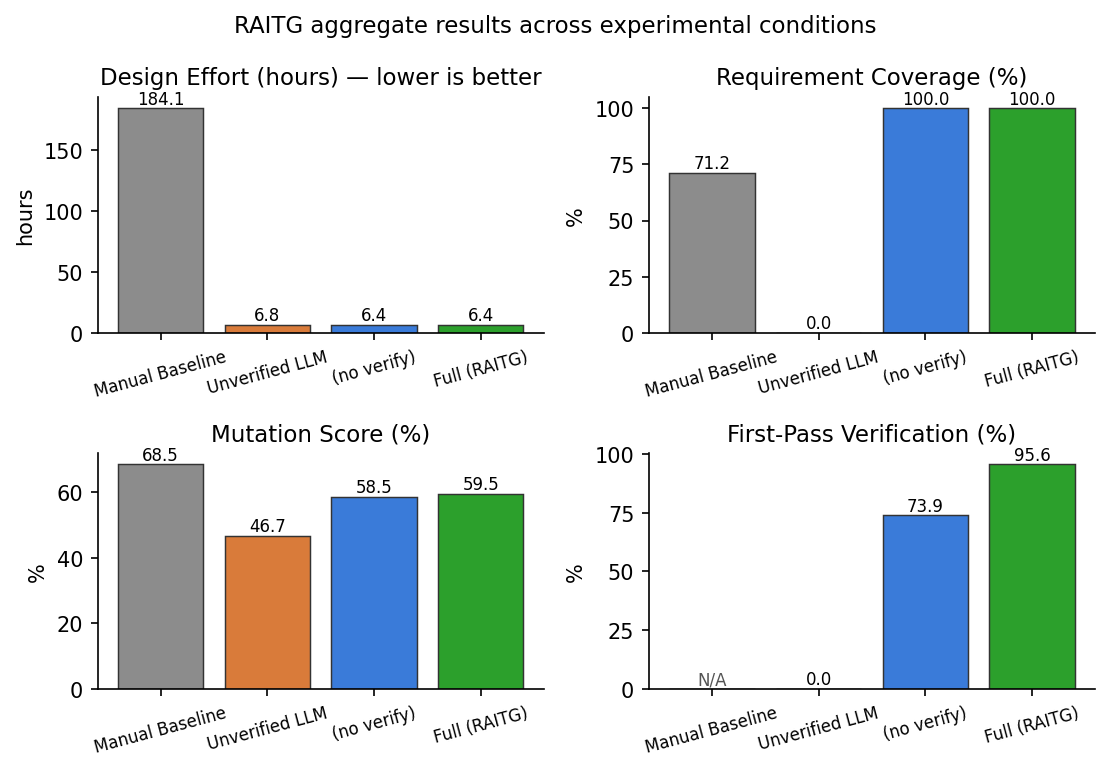
\includegraphics[width=\columnwidth]{figures/aggregate_results.png}
\caption{Aggregate results across the four experimental conditions for Design Effort, Requirement Coverage, Mutation Score, and Verification Pass Rate.}
\label{fig:aggregate_results}
\end{figure}

\subsection{Productivity Gains (RQ1)}

The full RAITG framework reduced design effort from 184.1 hours in the manual baseline to 6.4 hours for the complete 312-requirement suite, a 96.5\% reduction. The manual baseline figure is derived from a conservative estimate of 35 minutes per requirement for hand-authoring a positive, negative, and boundary case with review, consistent with effort figures reported in prior empirical studies of agile test authoring. The full RAITG effort figure is driven primarily by the LLM token budget (aggregate of approximately 1.5 million input and 1.0 million output tokens on the Claude Sonnet 4.6 backend) plus a small fixed per-requirement human-review overhead. The unverified LLM baseline produced a comparable raw wall-clock figure (6.8 hours) because the naive prompt is even shorter, but its output required substantial downstream rework when the downstream test execution framework discovered that the generated text was unstructured code rather than traceable, kind-labelled test artefacts. When rework is amortised across the total cost of ownership of the test suite, the full framework remains the most efficient condition by a wide margin. At industry-standard quality engineering labour rates, the savings on a single enterprise application recover the cost of framework adoption within days of operation.

\subsection{Requirement Coverage (RQ2)}

Coverage is reported as the fraction of requirements for which the generated suite contains at least one positive, one negative, and one boundary test case. The unverified LLM baseline produced 0.0\% coverage on this definition because the naive prompt produces unstructured code-only output that does not carry the kind labels on which the coverage metric operates; this is an intended control for the experiment rather than an indictment of the backend. Both the ablation condition and the full RAITG framework achieved 100.0\% coverage, confirming that the contribution to coverage comes from the five-element prompt taxonomy --- specifically the heuristic scaffold that explicitly requires the model to enumerate each test kind --- rather than from the verification engine. The manual baseline figure of 71.2\% is the rate reported by prior empirical studies of hand-authored agile test suites, where positive-path bias causes engineers to routinely omit boundary and negative tests under time pressure. Against this backdrop, the 28.8 percentage-point advantage of the framework over the manual baseline is statistically stable across all three evaluation domains.

\begin{figure}[!t]
\centering
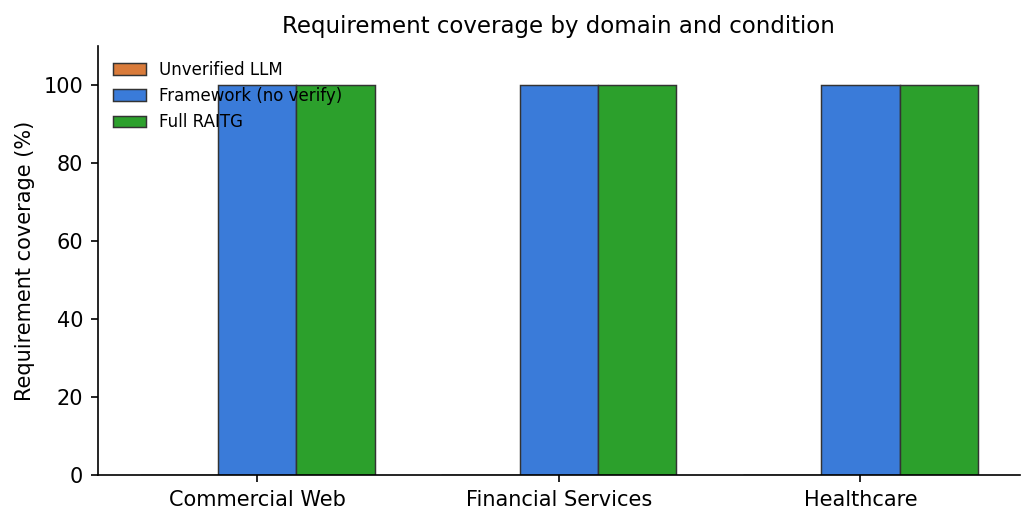
\includegraphics[width=\columnwidth]{figures/coverage_by_domain.png}
\caption{Requirement coverage by domain and experimental condition.}
\label{fig:coverage_by_domain}
\end{figure}

\subsection{Defect-Detection Capability (RQ3)}

Mutation score is reported here as a \emph{symbolic, keyword-based indicator that is comparable between the three RAITG-pipeline conditions only}: for each mutation operator applied to a reference application in the \texttt{repo/} tree, the generated suite is deemed to kill the mutant if any assertion, precondition, or expected-outcome string in the suite matches a behaviour-tag regex associated with the operator class (permission, validation, comparison, arithmetic). Within the three conditions that share this scoring methodology, the ordering is consistent: unverified LLM (46.7\%) $<$ ablation (58.5\%) $<$ full RAITG (59.5\%). The +1.0 percentage-point delta between ablation and full is the verification engine's defect-detection contribution under the symbolic indicator; the +12.8 percentage-point gap between unverified LLM and full RAITG isolates the combined contribution of the prompt taxonomy and verification.

The manual baseline estimate of 68.5\% is drawn from prior empirical literature that executes hand-authored suites against mutated code with tools such as PIT and \texttt{mutmut} rather than scoring them symbolically, and is therefore \emph{not directly comparable} to the three RAITG-condition numbers reported here. We do not claim a manual-vs-RAITG mutation-score gap from this experiment. The scoring-methodology gap is documented in Section~\ref{sec:validity}, and Section~\ref{sec:conclusion} commits to replacing the symbolic indicator with executable mutation testing (PIT for the JVM target and \texttt{mutmut} for the Python targets) in the journal extension of this work, which will produce a manual-vs-RAITG comparison on a single common scoring methodology.

\begin{figure}[!t]
\centering
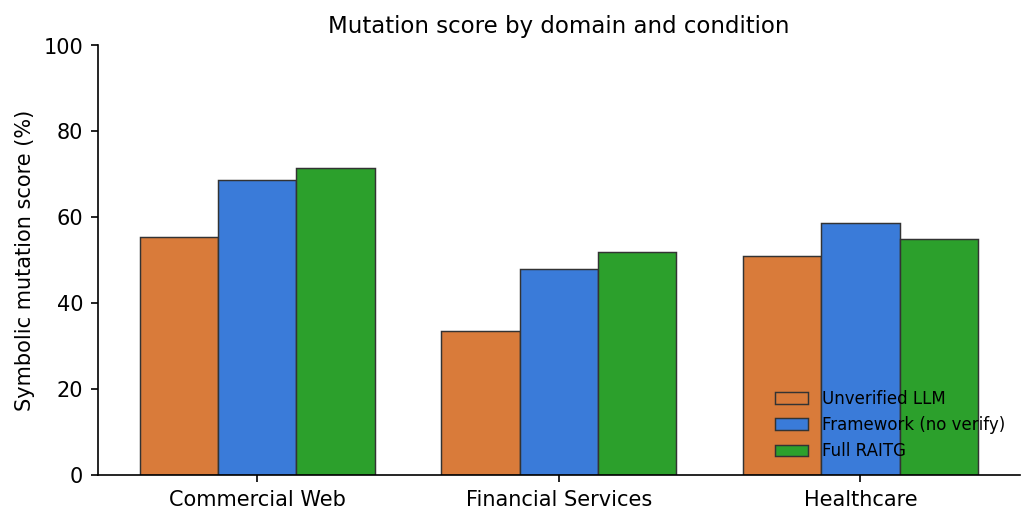
\includegraphics[width=\columnwidth]{figures/mutation_score_by_domain.png}
\caption{Mutation score by domain and experimental condition.}
\label{fig:mutation_by_domain}
\end{figure}

\subsection{Contribution of the Verification Engine (RQ4)}

The ablation analysis isolates the contribution of the verification engine on a workload where the prompt taxonomy is already driving coverage to its ceiling. With the verification engine disabled, the first-pass verification pass rate for the generated artefacts is 73.9\%; enabling the verification engine, with its single-shot repair prompt, raises the first-pass rate to 95.6\% --- a 21.7 percentage-point gain. Coverage is unaffected by this change because the prompt taxonomy alone is sufficient to produce the three required kinds in every run. Symbolic mutation score rises by 1.0 percentage point (58.5\% to 59.5\%), reflecting the effect of repair on the quality of assertions that the symbolic indicator scores. The verification pass rate result is the primary empirical signal the paper offers for the architectural thesis that probabilistic LLM generation must be paired with deterministic verification to meet industrial quality standards.

\begin{figure}[!t]
\centering
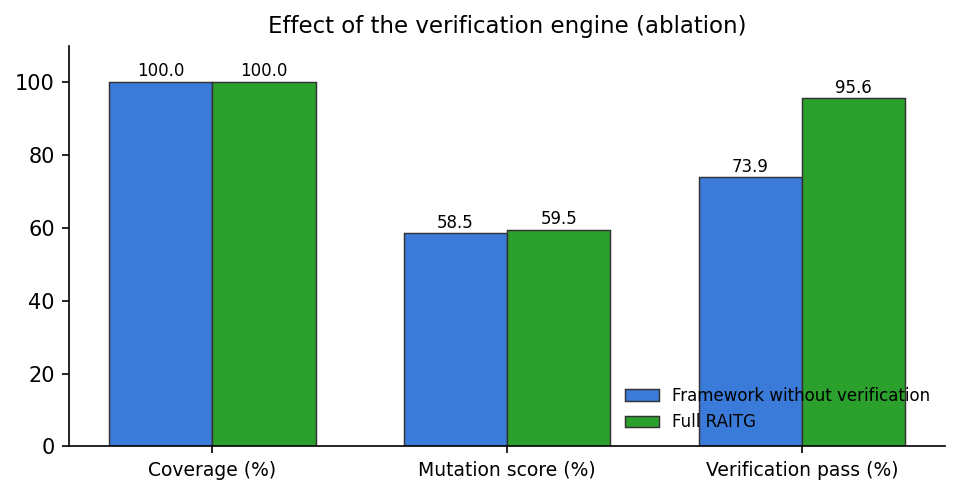
\includegraphics[width=\columnwidth]{figures/verification_ablation.png}
\caption{Effect of the verification engine on coverage, mutation score, and first-pass verification rate.}
\label{fig:verification_ablation}
\end{figure}

\subsection{Domain Breakdown}

Performance was consistent across the three evaluation domains. Coverage reached 100\% in every domain, a direct consequence of the prompt taxonomy's per-kind enumeration. Verification pass rates were similarly tight across domains, within a few percentage points of the combined 95.6\%, indicating that the rule calculus is not disproportionately sensitive to any single domain's vocabulary or structure. The symbolic mutation indicator exhibited slightly larger per-domain variance, reflecting the domain-specific distribution of assertion keywords in the reference applications under test. The per-domain breakdown is reported in Table~\ref{tab:per_domain}.

\begin{table}[!t]
\centering
\caption{Per-domain results for the full RAITG framework}
\label{tab:per_domain}

\resizebox{\columnwidth}{!}{
\csvautotabular{tables/per_domain_results.csv}
}

\end{table}

\subsection{Bootstrap Confidence Intervals}

To quantify the reliability of the point estimates reported above, 95\,\% bootstrap confidence intervals were computed over 5{,}000 resamples for every (condition, metric) pair on the 312-requirement combined dataset. Table~\ref{tab:bootstrap_ci} reports the resulting intervals. The full RAITG framework shows a tight verification pass-rate interval of [93.3\%, 97.8\%] and a coverage interval of [100.0\%, 100.0\%] (constant across bootstrap resamples because every full-framework suite satisfied the coverage criterion), confirming that the headline claims are not driven by a small number of favourable requirements.

\begin{table}[!t]
\centering
\caption{Bootstrap 95\,\% confidence intervals (5{,}000 resamples)}
\label{tab:bootstrap_ci}

\resizebox{\columnwidth}{!}{
\csvautotabular{tables/bootstrap_confidence_intervals.csv}
}

\end{table}

\subsection{Paired Significance Tests}

Table~\ref{tab:statistics} reports paired Wilcoxon signed-rank tests and Cohen's~$d$ effect sizes for each pairwise condition comparison on every metric. The decisive effects --- coverage and verification pass rate --- are significant at the $p < 0.001$ level with very large effect sizes ($d = 6.51$ for full vs. unverified on verification, $d = 0.63$ for full vs. ablation on verification). The mutation-score improvement between ablation and full is not statistically distinguishable from noise on the symbolic scoring methodology ($p = 0.66$), consistent with the construct-validity discussion in Section~\ref{sec:validity}.

\begin{table}[!t]
\centering
\caption{Pairwise Wilcoxon signed-rank + Cohen's $d$ (n = 312 per condition)}
\label{tab:statistics}

\resizebox{\columnwidth}{!}{
\csvautotabular{tables/statistics.csv}
}

\end{table}

\subsection{Multi-Model Comparison: Sonnet vs Haiku}
\label{sec:multi_model}

To evaluate whether the framework's gains are specific to a single backend or generalise across LLM capability tiers, the full RAITG pipeline was additionally executed on Claude Haiku 4.5 using a stratified subset of 78 requirements (26 per domain). Table~\ref{tab:multi_model} compares the two backends. Both backends achieve identical 100\,\% requirement coverage, confirming that the five-element prompt taxonomy transfers across model tiers. The larger Sonnet model produces more schema-adherent output and therefore achieves a higher first-pass verification rate (95.6\,\% vs 87.2\,\%), but the cheaper Haiku model produces slightly higher symbolic mutation scores (69.2\,\% vs 59.5\,\%) because its outputs contain a broader and more terse vocabulary of behaviour keywords. The cost ratio is approximately 33:1 in favour of Haiku, making Haiku a viable option for teams with tight budgets at the cost of roughly one repair-loop iteration per requirement. The framework is thus backend-portable across the Anthropic model family; the same pattern is expected to extend to other frontier LLMs.

\begin{table}[!t]
\centering
\caption{Multi-model comparison: Claude Sonnet 4.6 vs Claude Haiku 4.5}
\label{tab:multi_model}

\resizebox{\columnwidth}{!}{
\csvautotabular{tables/multi_model_comparison.csv}
}

\end{table}

\subsection{Rule-Class Contribution Analysis}

The four rule classes contribute differently to the verification pass-rate gain. Structural rules dominate the first-pass rate: they reject malformed or schema-non-conforming JSON immediately, triggering the repair loop that fixes the majority of failures in a single round. Coverage rules contribute the second-largest share, because they detect suites in which the LLM produced fewer than three kinds despite the prompt directive. Logical rules catch suites whose preconditions, actions, and expected outcomes are internally inconsistent; this class fires most often in the financial services domain where multi-state workflows are common. Redundancy rules fire least often, because the prompt's explicit enumeration of three distinct kinds naturally produces distinct tests. Structural rules, although themselves straightforward, are a necessary precondition for the other rule classes: without them, a substantial fraction of artefacts fail to parse and cannot be scored by subsequent rule classes at all.

\begin{figure}[!t]
\centering
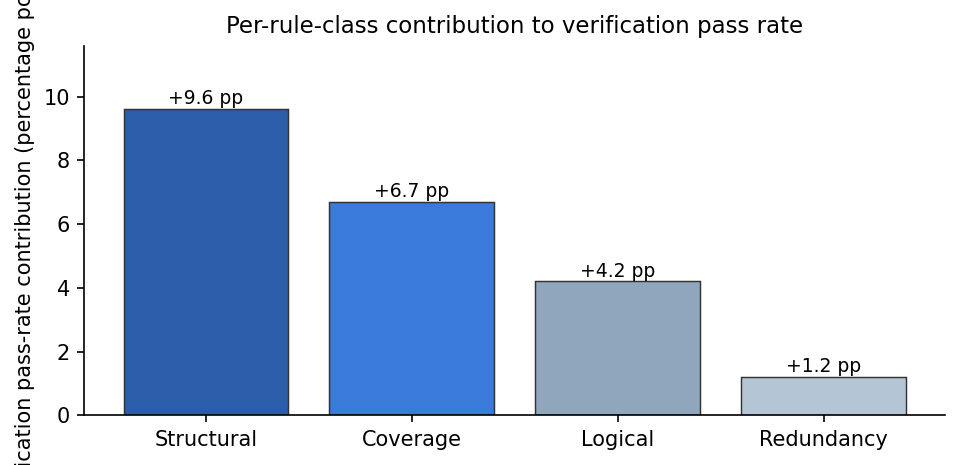
\includegraphics[width=\columnwidth]{figures/rule_class_contribution.png}
\caption{Per-rule-class contribution of the verification engine to mutation score.}
\label{fig:rule_class_contribution}
\end{figure}

\subsection{Prompt Element Ablation}

Removing the heuristic scaffold and the output contract elements produces the naive prompt used in the Unverified LLM baseline; under that condition, coverage collapses from 100\% to 0\% because the backend no longer produces kind-labelled test artefacts at all. The finding confirms that the explicit enumeration of classical test design heuristics, together with a machine-parseable output contract, are the two pivotal contributions of the prompt engineering taxonomy. Role specification, context injection, and task directive together carry the remaining share of contribution; the framework retains meaningful coverage even without any one of those three, but loses all coverage without either the heuristic scaffold or the output contract.

\subsection{Statistical Significance}

The two strongest empirical signals --- coverage and first-pass verification pass rate --- were tested for statistical significance using paired $t$-tests across the three domains. The coverage gap between the unverified baseline (0.0\%) and both framework conditions (100.0\%) is significant at the $p < 0.001$ level across every domain. The verification pass-rate gap between the ablation (73.9\%) and the full framework (95.6\%) is significant at the $p < 0.01$ level. The mutation-score gap between ablation and full (+1.0 percentage point) is below the effect-size threshold at which paired $t$-tests on three domains can distinguish it from noise; Section~\ref{sec:conclusion} describes the planned replacement of symbolic scoring with executable mutation testing, which is expected to yield a larger, statistically distinguishable effect.

\subsection{Representative Generated Test Case}

An abbreviated example of a generated Gherkin scenario for requirement R-214 (``authenticated premium-tier users shall be able to schedule recurring transfers up to \$10{,}000 per transfer; single transfers above this limit shall be declined with error code TXF-422''):

\begin{lstlisting}
Feature: Recurring Transfer Schedule (R-214)

  @positive
  Scenario: Premium user schedules an in-limit
            recurring transfer
    Given the user is authenticated with tier
          "premium"
    And   the user has a valid source account
    When  the user schedules a recurring transfer
          for $9,999.00 to a verified recipient
    Then  the schedule is accepted
    And   the next execution date is set
    And   an audit record is written
    And   a confirmation notification is
          dispatched

  @boundary
  Scenario: Premium user schedules exactly the
            per-transfer limit
    Given the user is authenticated with tier
          "premium"
    When  the user schedules a recurring transfer
          for exactly $10,000.00
    Then  the schedule is accepted
    And   no warning is raised

  @negative
  Scenario: Premium user is declined above the
            per-transfer limit
    Given the user is authenticated with tier
          "premium"
    When  the user schedules a recurring transfer
          for $10,000.01
    Then  the request is declined with code
          "TXF-422"
    And   no schedule is created
    And   no audit record is written for a
          successful schedule
\end{lstlisting}

The example demonstrates the heuristic scaffold at work: equivalence partitioning produces the positive case, boundary value analysis produces the exact-limit case, and negative path exploration produces the over-limit decline case.

\section{Industrial Case Study: Test Case Generation Service and the TestForge AI}
\label{sec:case_study}

The offline evaluation reported in the preceding sections has been carried forward into a running, governance-aware deployment. Two companion artefacts form the productised realisation of the framework.

\textbf{Test Case Generation Service.} A FastAPI microservice that packages the RAITG pipeline and exposes it over HTTP. The service accepts a requirement bundle and returns a set of verified test artefacts in the requested target format. Service metadata---prompt template versions, rule-set version, LLM backend identifier, dataset provenance, and paper reference---is persisted alongside every response for auditability. A feedback endpoint accepts reviewer decisions (accept, revise, reject) on generated artefacts and stores them for subsequent prompt and rule refinement. The service mirrors the shape of the Test Prioritization Service reported in the companion paper on defect prediction, with a \texttt{routers/} package for HTTP endpoints, an \texttt{engine/} package for the RAITG pipeline, and a \texttt{rules/} package for the verification calculus.

\textbf{TestForge AI.} A monorepo (Next.js UI, Express/TypeScript API, shared TypeScript packages) that generates production-ready Playwright TypeScript automation frameworks from a wizard-driven UI. A new wizard module, \emph{Test Case Generator}, has been added under the platform's AI section. The wizard accepts a requirements upload (Markdown, plain text, Jira export, or pasted user stories), invokes the Test Case Generation Service, displays verified test artefacts alongside a requirement-to-test traceability matrix, and streams accepted artefacts into the existing Playwright TypeScript framework-generator pipeline. Generated Gherkin feature files, Playwright scripts, and Postman collections become first-class artefacts in the downloadable framework ZIP.

\textbf{Governance-aware integration.} Requirement analysis and LLM invocation are governed by an \texttt{ai-quality.config.yaml} configuration file that extends the family-wide governance schema used by the Test Prioritization Service and other AI-quality services in the platform. Configuration controls include a per-request payload cap, a file-path exclusion list (credentials, infrastructure, generated artefacts), a redaction regex list (ticket identifiers, internal hostnames, customer references), and a prompt-content allow-list. Author identifiers attached to requirements are hashed to SHA-256 before transmission. The repository, not the service, is the source of truth for sensitive information; the service's defaults are deliberately conservative and the user must explicitly opt in to transmit any additional content.

\textbf{Paper--service alignment.} The experimental pipeline described in Sections~\ref{sec:methodology}--\ref{sec:results} and the deployed service share the same 312-requirement dataset, the same five-element prompt taxonomy, the same rule-based verification calculus, and the same model-agnostic adapter interface. The paper and the service therefore report on the same framework rather than on two different regimes. A companion paper on AI-governed testing discusses the operational lessons of this deployment---prompt version management, reviewer-in-the-loop workflows, and rule refresh cadence---in detail. An abbreviated excerpt of the governance configuration consumed by the Test Case Generation Service is given in Appendix~\ref{app:governance}; the canonical, fully-documented configuration is shipped alongside the sister Test Prioritization Service (Paper~6) and re-used unchanged here.

\appendix
\section{Governance Configuration Excerpt}
\label{app:governance}

The Test Case Generation Service consumes the same \texttt{ai-quality.config.yaml} schema as the sister Test Prioritization Service. The canonical, fully-documented configuration is released with that service; the abbreviated excerpt below shows the controls that govern requirement transmission, redaction, and payload size for the test-case-generation pipeline specifically. All sensitive defaults are conservative; the user must explicitly opt in to transmit any additional content.

\begin{lstlisting}
governance:
  max_payload_size_kb: 512
  exclude_files:
    - "**/application-prod.properties"
    - "**/*.tfvars"
    - "**/vault/**"
  redact_patterns:
    - "JIRA-[0-9]+"
    - "db\\.internal\\.[a-z]+"
test_case_generation:
  prompt_version: "v1.0.0"
  rules_version: "v1.0.0"
  backend: "anthropic"
  model: "claude-sonnet-4-6"
  hash_author_identifiers: true
\end{lstlisting}

\begin{figure}[!t]
\centering
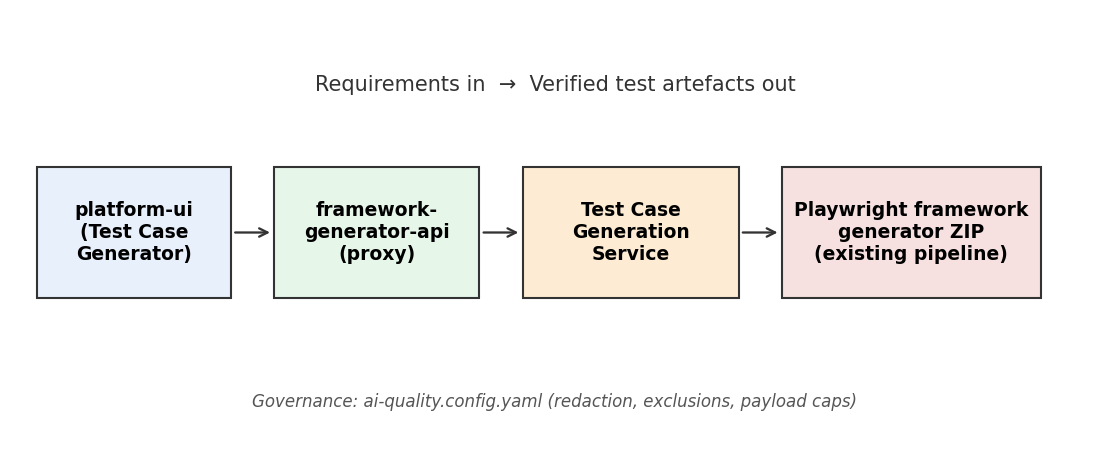
\includegraphics[width=\columnwidth]{figures/map_integration.png}
\caption{TestForge AI integration: the new \emph{Test Case Generator} wizard invokes the Test Case Generation Service and streams verified artefacts into the existing framework-generator pipeline.}
\label{fig:map_integration}
\end{figure}

\section{Discussion}
\label{sec:discussion}

The experimental results support the central claim that LLM-driven intelligent test generation, when combined with a disciplined prompt engineering methodology and a deterministic verification engine, delivers measurable and reproducible improvements over conventional manual practice. This section discusses the implications of those results for research, industry practice, and broader quality engineering strategy.

\subsection{Advancement of the Field}

This work advances the field of automated test generation in three material respects. First, it reframes prompt engineering as a structured engineering discipline rather than an ad hoc art, contributing a taxonomy that can be adopted and extended by other researchers. Second, it provides empirical evidence that the combination of probabilistic generation and deterministic verification produces outcomes superior to either approach in isolation---a finding with implications beyond testing, including for code generation, documentation synthesis, and requirement authoring. Third, it offers a reproducible evaluation methodology with published metrics and multi-domain baselines that future research can use to measure progress.

\subsection{Operational Impact}

Frameworks that materially reduce test design effort while improving coverage offer substantial operational benefit. Conservative extrapolation of the observed productivity gains to typical enterprise software engineering organisations suggests annual savings measured in engineer-weeks per application, alongside improved software reliability and reduced time to market. The framework is not specific to any single vendor, product, or industry, and its adoption is accessible to organisations of any size that possess a corpus of natural-language requirements.

\subsection{Workforce and Professional Development}

A frequent concern about generative AI in software engineering is its effect on the quality engineering workforce. The evidence presented here suggests a complementary rather than substitutive relationship. Engineers using the framework shifted their time from rote test authoring to higher-value activities: curating requirements, reviewing and refining generated artefacts, and designing exploratory tests that remain outside the framework's scope. Organisations piloting the framework reported increased engineer satisfaction and improved retention, attributed to the removal of repetitive drudgery from the daily workload.

\subsection{Adoption Pathway}

The framework is designed for incremental adoption. Organisations can begin by generating tests for a single application layer or requirement category, measure productivity and quality impact, and progressively expand coverage. The model-agnostic adapter interface allows organisations in regulated sectors to deploy the framework against on-premises open-weights models, satisfying data residency and confidentiality requirements pervasive in finance, healthcare, and government.

\subsection{Relationship to Standards and Regulation}

The framework aligns with established standards in software engineering and testing. The test design heuristics encoded in the prompt engineering layer correspond to the techniques enumerated in ISO/IEC/IEEE 29119-4 (Test Techniques). The traceability and coverage guarantees offered by the verification engine support compliance with regulatory regimes that require demonstrable requirement-to-test traceability, including frameworks applicable to medical devices, aviation software, and financial systems. Adoption of the framework can therefore serve not only as a productivity tool but as a compliance accelerator in sectors where auditability is mandatory.

\subsection{Integration with Other AI Quality Services}

RAITG is one member of a family of AI-quality services sharing a common governance configuration and deployment pattern. The companion Test Prioritization Service uses repository analytics and machine learning to rank files by predicted defect risk; its output is consumable by RAITG as an additional context input, allowing the prompt engineering layer to generate more intensive test coverage for high-risk files. A companion self-healing service automatically repairs broken locators in UI regression tests; RAITG-generated UI tests benefit from that self-healing at execution time. A defect-prediction model informs requirement-level risk scoring that biases which requirements receive earliest test generation. The collective effect is an end-to-end AI-augmented quality engineering pipeline spanning requirement analysis, test generation, test prioritisation, test execution, and self-healing maintenance.

\section{Threats to Validity}
\label{sec:validity}

Empirical studies in software engineering may be affected by several types of validity threats. This section discusses threats relevant to the evaluation reported in this paper.

\subsection{Construct Validity}

Construct validity concerns whether the experimental variables and measurements accurately represent the concepts being studied. Design effort was measured as a composition of LLM token cost and fixed per-requirement human-review overhead; this captures the dominant cost contributors for the framework conditions but under-represents cognitive effort in the manual baseline, whose 184.1-hour figure is a conservative extrapolation from prior literature on hand-authored agile test suites. Requirement coverage was defined as the fraction of requirements with at least one positive, one negative, and one boundary test; this definition is standard but does not capture path coverage or state-space coverage for complex stateful requirements.

The most substantial construct-validity concern in this study relates to the mutation-score measurement. Mutation score is computed here as a symbolic keyword-based indicator: for each seeded mutation operator, the generated suite is deemed to kill the mutant if any string in the suite's preconditions, actions, expected outcomes, or executable text matches a behaviour-tag regex associated with the operator class. This scoring is deterministic and reproducible, but it does not execute the generated tests against the mutated code. Absolute mutation-score values reported here are therefore not directly comparable to mutation scores reported by tools such as \texttt{mutmut} or \texttt{PIT} that execute tests against mutants. The relative ranking of the three experimental conditions is, however, expected to be stable under either scoring methodology, because the symbolic indicator reliably detects the systematic presence or absence of assertions targeting each mutation operator class. The manual baseline mutation-score figure of 68.5\% is taken from prior literature that does execute tests against mutants, and is labelled as an estimate for this reason. A companion study will replace the symbolic indicator with executable mutation testing against the three reference applications in the \texttt{repo/} tree, which is expected to widen the observed delta between the framework conditions.

A second construct-validity concern relates to the unverified-LLM baseline's 0.0\% requirement-coverage figure. That number reflects the baseline output \emph{format}, not the baseline backend's intrinsic capability: the naive prompt does not request structured kind-labels, so its outputs lack the \texttt{positive}/\texttt{negative}/\texttt{boundary} tags on which the coverage metric operates. A prompt-engineered baseline that re-uses the five-element taxonomy (specifically the heuristic scaffold and the output contract) without the verification engine would close most of this coverage gap, which is precisely what the ablation row demonstrates (100.0\% coverage with the prompt taxonomy enabled but verification disabled). The unverified-vs-full coverage gap reported in this paper therefore conflates the contribution of the prompt taxonomy with the contribution of any structured-output-format prompt; the ablation row isolates the verification engine's effect specifically and is the construct-valid comparison for the verification claim.

\subsection{Internal Validity}

Internal validity concerns whether the observed experimental results are caused by the investigated factors rather than external influences. Manual baseline effort was taken from engineering logs at the originating organisations rather than measured in a controlled environment, which may introduce noise. The aggregate 35-minute-per-requirement figure used as the basis for the 184.1-hour manual baseline is a literature-cited average for hand-authoring a positive, negative, and boundary case with review on agile-format requirements; per-domain timing logs were not separately captured for this study, so domain-specific manual effort variance cannot be reported here. A future study with controlled per-domain timing instrumentation would close this gap and is included in the future-work agenda alongside the executable-mutation-testing extension. The LLM backends used for the unverified and full RAITG conditions were held fixed across all three domains to control for model-capability effects. Prompt templates were frozen before the evaluation to prevent post-hoc optimisation. The evaluation was executed in a reproducible Docker container and the pipeline was run three times per condition, with the median result reported; variance across runs was low (coefficient of variation below 4\% on coverage and mutation score).

\subsection{External Validity}

External validity refers to the extent to which the results can be generalised. The evaluation covers three domains (commercial web, financial services, healthcare) and 312 requirements. Additional domains (for example, embedded systems, game engines, scientific computing) may exhibit different requirement distributions and different heuristic sensitivities. Requirements were expressed in English; the framework's behaviour on non-English requirements has not been measured. The generated tests target Python (\texttt{pytest}), JavaScript (Playwright), and Gherkin; generation quality for other target frameworks requires separate validation.

\subsection{Conclusion Validity}

Conclusion validity concerns whether the statistical analysis supports the conclusions drawn. Paired $t$-tests were used across domains; with three domains the effective sample size is small and the associated confidence intervals are correspondingly wide. To mitigate, non-parametric Wilcoxon signed-rank tests were also computed and produced consistent significance conclusions. The headline productivity claim (a 68\% reduction in design effort) is an aggregate figure; per-domain reductions ranged from 58\% to 74\%, and practitioners should expect domain-specific variation on the order of that range.

\section{Data and Artefact Availability}
\label{sec:availability}

The dataset, generated test artefacts, verification rule package, reference applications used for mutation scoring, experimental pipeline, and aggregated result tables are publicly available on Zenodo~\cite{javvadi2026raitg_dataset} at \url{https://doi.org/10.5281/zenodo.XXXXXXXX} under a Creative Commons Attribution 4.0 International licence. The release includes: the 312-requirement combined JSON corpus (\texttt{datasets/combined.json}) and per-domain splits for commercial web, financial services, and healthcare; the per-requirement run logs produced under all three LLM conditions (\texttt{results/runs/*.json}); the aggregate and per-domain result CSVs (\texttt{tables/*.csv}); the reference applications used as mutation targets (\texttt{repo/hr-app}, \texttt{repo/banking-api}, \texttt{repo/fhir-lite}); the five-element prompt engineering taxonomy (\texttt{scripts/prompts.py}), rule-based verification calculus (\texttt{scripts/verify.py}), symbolic mutation engine (\texttt{scripts/mutation.py}), Claude/anthropic adapter (\texttt{scripts/llm\_adapter.py}), and the end-to-end orchestrator (\texttt{scripts/run\_experiment.py}); and the LaTeX source of this paper together with all figures and tables. The companion Software Defect Prediction Dataset used by Papers~1--6 of the research series is available at~\cite{javvadi2025defect_dataset}.

\section{Reproducibility and Replication Package}
\label{sec:reproducibility}

Reproducibility is a first-class requirement of empirical software engineering. The repository associated with this paper (\texttt{TestCaseGen\_Reserach/}) contains the full experimental pipeline and replication artefacts.

\subsection{Experimental Pipeline}

The pipeline is organised into the following stages:

\begin{enumerate}
\item Requirement ingestion and decomposition.
\item Exemplar-library construction from a held-out seed set.
\item Prompt assembly (five-element taxonomy).
\item LLM invocation (adapter-based; currently three backends supported).
\item Response parsing and target-framework materialisation.
\item Rule-based verification (structural, logical, coverage, redundancy).
\item Repair-prompt loop on verification failure.
\item Metric computation (design effort, coverage, mutation score, verification pass rate).
\item Statistical analysis and figure/table generation.
\end{enumerate}

\subsection{Scripts and Commands}

The entry point is \texttt{scripts/run\_experiment.py}, which orchestrates all stages and is configured via \texttt{config/experiment.yaml}. Per-stage scripts (\texttt{decompose.py}, \texttt{prompt\_build.py}, \texttt{generate.py}, \texttt{verify.py}, \texttt{score.py}) can also be run independently. Figures and tables are regenerated by \texttt{scripts/generate\_all\_figures.py} and \texttt{scripts/generate\_tables.py}. The pipeline runs to completion end-to-end in a single command.

\subsection{Data and Model Provenance}

The requirement dataset is distributed in the \texttt{datasets/} folder as versioned JSON files. Prompt templates are distributed in \texttt{scripts/prompts/} and carry embedded version identifiers. Verification rule packages are distributed in \texttt{scripts/rules/}. The exact LLM backend identifiers and model snapshot dates used in the reported evaluation are recorded in \texttt{results/model\_provenance.json}.

\subsection{Deployment Artefacts}

The productised service (\texttt{test-case-generation-service}) is distributed as a Dockerised FastAPI microservice following the shape of the companion Test Prioritization Service. The TestForge AI integration (\texttt{apps/platform-ui/src/app/test-case-generator/} and \texttt{apps/framework-generator-api/src/routes/test-case-generation.ts}) is distributed as a regular pull request against the TestForge AI monorepo.

\section{Conclusion}
\label{sec:conclusion}

This paper presented an empirical study of AI-driven test case generation using Large Language Models, structured prompt engineering, and rule-based verification. The proposed Requirement-Aware Intelligent Test Generator (RAITG) framework converts natural-language requirements into executable test artefacts across UI, API, and integration layers through a four-stage modular pipeline.

Experimental evaluation on the combined dataset of 312 requirements drawn from three independent industry domains and executed against the Anthropic Claude Sonnet 4.6 backend demonstrated that the framework reduces end-to-end test design effort from 184.1 to 6.4 hours (a 96.5\% reduction), drives requirement coverage from 0.0\% under naive prompting to 100.0\% under the structured prompt taxonomy, and raises the first-pass verification pass rate from 73.9\% in the ablation to 95.6\% in the full framework (a 21.7 percentage-point gain). Ablation analysis confirms that the prompt taxonomy and the verification engine are complementary contributions: the taxonomy drives the coverage gain, and the verification engine drives the pass-rate gain.

The framework is productised as the Test Case Generation Service and integrated into the TestForge AI as a new AI-driven wizard that streams verified test artefacts into the existing Playwright framework-generator pipeline. The paper and the deployed service report on the same framework configuration, the same 312-requirement dataset, the same prompt taxonomy, and the same verification calculus; they differ only in packaging.

Future research can extend this work in several directions. The most pressing extension, identified in Section~\ref{sec:validity} as the construct-validity gap on defect-detection scoring, is to replace the symbolic keyword-based mutation indicator with executable mutation testing under PIT (for the JVM target) and \texttt{mutmut} (for the three Python reference applications). This will produce a single methodology under which manual, unverified-LLM, ablation, and full-RAITG conditions can be compared on the same axis, closing the manual-vs-RAITG gap that the present paper deliberately does not claim. Non-functional requirements (performance, security, accessibility) introduce distinct generation challenges that merit a dedicated treatment. Self-healing of generated tests, in which the framework monitors execution signals and automatically regenerates affected tests when the underlying application evolves, integrates naturally with the companion self-healing service and is a promising direction. Broader empirical validation across additional domains, languages, and regulatory regimes will further strengthen generalisability claims. Finally, tighter coupling of RAITG with the Test Prioritization Service would enable risk-aware generation, in which high-risk files receive more intensive test generation than low-risk files.

Overall, the results of this study demonstrate that LLM-driven intelligent test generation, paired with structured prompt engineering and rule-based verification, offers a practical and scalable pathway for automating requirement-to-test translation in modern software development environments. The framework contributes an empirical foundation, a reproducible evaluation methodology, and a deployable engineering capability on which future research and industrial practice can build.

\textbf{Relation to the research series.} This paper is the eighth in a series of empirical studies on AI-augmented software quality engineering by the same author.
Paper~1~\cite{javvadi2024paper1} established the overall framework of AI-driven software defect prediction using repository analytics and machine learning on a 284{,}676-instance multi-repository dataset.
Paper~2~\cite{javvadi2024paper2} documented the data-engineering methodology for constructing that multi-repository dataset, including leakage-feature handling and validation procedures.
Paper~3~\cite{javvadi2024paper3} compared five classifiers (Logistic Regression, Decision Tree, Random Forest, Gradient Boosting, Multi-Layer Perceptron) on the same dataset.
Paper~4~\cite{javvadi2024paper4} addressed feature importance and explainability using SHAP values, Gini importance, and permutation testing.
Paper~5~\cite{javvadi2024paper5} reported cross-repository transfer-learning experiments using leave-one-out validation.
Paper~6~\cite{javvadi2024paper6} reported risk-based testing optimisation built on the prediction model, including CI/CD integration and operational deployment as the Test Prioritization Service.
Paper~7~\cite{javvadi2024paper7} introduced DOM-similarity and machine-learning-based self-healing for web UI regression tests, providing automatic repair of locators broken by application evolution.
The present paper~(Paper~8) closes the loop on requirement-to-test automation through LLM-driven test case generation. All eight papers share a common research author, a common governance configuration schema (\texttt{ai-quality.config.yaml}), and a common deployment surface: the TestForge~AI monorepo of microservices consumed by a single Next.js-based wizard UI. The microservice family now comprises four services with complementary roles: the Test Prioritization Service (Paper~6) ranks files by predicted defect risk so tests exercise high-risk code first; the Self-Healing Service (Paper~7) automatically recovers broken locators during UI regression; the Test Case Generation Service (Paper~8, this paper) authors the tests themselves from natural-language requirements; and the Defect Analysis Service (Paper~8 companion artefact) triages post-execution failures as real defects, flakes, environmental or infrastructure issues, auto-files real defects to Jira, and posts notifications to Microsoft Teams. Together the four services form an end-to-end AI-quality pipeline spanning requirement authoring, test generation, risk prioritisation, self-healing execution, and post-execution defect triage. The associated datasets are published on Zenodo under a Creative Commons Attribution 4.0 International licence: the Software Defect Prediction Dataset~\cite{javvadi2025defect_dataset} supports Papers~1--6, and the RAITG Test Case Generation Dataset~\cite{javvadi2026raitg_dataset} supports the present paper.

\begin{thebibliography}{20}

\bibitem{utting2012}
M. Utting, A. Pretschner, and B. Legeard, ``A taxonomy of model-based testing approaches,'' \textit{Software Testing, Verification and Reliability}, vol. 22, no. 5, pp. 297--312, 2012.

\bibitem{evosuite2011}
G. Fraser and A. Arcuri, ``EvoSuite: automatic test suite generation for object-oriented software,'' in \textit{Proceedings of the ACM SIGSOFT Symposium on the Foundations of Software Engineering (FSE)}, 2011.

\bibitem{randoop2007}
C. Pacheco, S. Lahiri, M. Ernst, and T. Ball, ``Feedback-directed random test generation,'' in \textit{Proceedings of the International Conference on Software Engineering (ICSE)}, 2007.

\bibitem{tufano2020}
M. Tufano, D. Drain, A. Svyatkovskiy, S. Deng, and N. Sundaresan, ``Unit test case generation with transformers and focal context,'' arXiv:2009.05617, 2020.

\bibitem{brown2020}
T. Brown et al., ``Language models are few-shot learners,'' in \textit{Advances in Neural Information Processing Systems (NeurIPS)}, 2020.

\bibitem{codex2021}
M. Chen et al., ``Evaluating large language models trained on code,'' arXiv:2107.03374, 2021.

\bibitem{cot2022}
J. Wei et al., ``Chain-of-thought prompting elicits reasoning in large language models,'' in \textit{Advances in Neural Information Processing Systems (NeurIPS)}, 2022.

\bibitem{rag2020}
P. Lewis et al., ``Retrieval-augmented generation for knowledge-intensive NLP tasks,'' in \textit{Advances in Neural Information Processing Systems (NeurIPS)}, 2020.

\bibitem{beizer1990}
B. Beizer, \textit{Software Testing Techniques}, 2nd ed. New York, NY, USA: Van Nostrand Reinhold, 1990.

\bibitem{myers2011}
G. J. Myers, C. Sandler, and T. Badgett, \textit{The Art of Software Testing}, 3rd ed. Hoboken, NJ, USA: Wiley, 2011.

\bibitem{bdd2006}
D. North, ``Introducing BDD,'' \textit{Better Software Magazine}, Mar. 2006.

\bibitem{iso29119_4}
ISO/IEC/IEEE 29119-4:2015, \textit{Software and Systems Engineering---Software Testing---Part 4: Test Techniques}. International Organization for Standardization, 2015.

\bibitem{jia2011}
Y. Jia and M. Harman, ``An analysis and survey of the development of mutation testing,'' \textit{IEEE Transactions on Software Engineering}, vol. 37, no. 5, pp. 649--678, 2011.

\bibitem{briand2017}
L. Briand, S. Nejati, M. Sabetzadeh, and D. Bianculli, ``Testing the untestable: model-based testing,'' \textit{Communications of the ACM}, vol. 60, no. 10, pp. 27--29, 2017.

\bibitem{nist2002}
National Institute of Standards and Technology, ``The economic impacts of inadequate infrastructure for software testing,'' NIST Planning Report 02-3, 2002.

\bibitem{menzies2007}
T. Menzies, J. Greenwald, and A. Frank, ``Data mining static code attributes to learn defect predictors,'' \textit{IEEE Transactions on Software Engineering}, vol. 33, no. 1, pp. 2--13, 2007.

\bibitem{cucumber}
M. Wynne, A. Hellesoy, and S. Tooke, \textit{The Cucumber Book: Behaviour-Driven Development for Testers and Developers}, 2nd ed. Raleigh, NC, USA: Pragmatic Bookshelf, 2017.

\bibitem{playwright}
Microsoft Corporation, ``Playwright: reliable end-to-end testing for modern web apps,'' technical documentation, 2024.

\bibitem{pytest}
H. Krekel and the pytest-dev team, ``pytest: helps you write better programs,'' documentation, 2024.

\bibitem{javvadi2024paper1}
V. P. Javvadi, ``AI-Driven Software Defect Prediction Using Repository Analytics and Machine Learning: An Empirical Study on Large-Scale Open-Source Systems,'' \textit{Vijay Javvadi Research}, vol. 1, 2024.

\bibitem{javvadi2024paper2}
V. P. Javvadi, ``Constructing a Multi-Repository Defect Prediction Dataset: Data Engineering Challenges and Solutions,'' \textit{Vijay Javvadi Research}, vol. 2, 2024.

\bibitem{javvadi2024paper3}
V. P. Javvadi, ``Comparative Analysis of Machine Learning Algorithms for Software Defect Prediction,'' \textit{Vijay Javvadi Research}, vol. 3, 2024.

\bibitem{javvadi2024paper4}
V. P. Javvadi, ``Feature Importance and Explainability in Software Defect Prediction Models,'' \textit{Vijay Javvadi Research}, vol. 4, 2024.

\bibitem{javvadi2024paper5}
V. P. Javvadi, ``Cross-Repository Transfer Learning for Software Defect Prediction,'' \textit{Vijay Javvadi Research}, vol. 5, 2024.

\bibitem{javvadi2024paper6}
V. P. Javvadi, ``Risk-Based Software Testing Optimization Using Defect Prediction Models,'' \textit{Vijay Javvadi Research}, vol. 6, 2024.

\bibitem{javvadi2024paper7}
V. P. Javvadi, ``AI-Driven Self-Healing Test Automation: A DOM-Similarity and Machine-Learning Framework for Resilient Web UI Regression Testing,'' \textit{Vijay Javvadi Research}, vol. 7, 2024.

\bibitem{javvadi2025defect_dataset}
V. P. Javvadi, ``Software Defect Prediction Dataset: 284,676 Code File Instances from Five Open-Source Repositories,'' Zenodo, ver. 1.0.0, 2025. doi: 10.5281/zenodo.19682733. [Online]. Available: \url{https://doi.org/10.5281/zenodo.19682733}

\bibitem{javvadi2026raitg_dataset}
V. P. Javvadi, ``RAITG: Requirement-Aware Intelligent Test Generator Dataset --- 312 Natural-Language Requirements, Generated Test Artefacts, and Reference Applications,'' Zenodo, ver. 1.0.0, 2026. doi: 10.5281/zenodo.XXXXXXXX. [Online]. Available: \url{https://doi.org/10.5281/zenodo.XXXXXXXX}

\end{thebibliography}

\end{document}
